\documentclass[10pt]{report}
\usepackage{epsf}
\usepackage{amsmath}
\usepackage{amssymb}
\usepackage{palatino}
\usepackage[pdftex]{graphics}
\usepackage{fancyhdr}
\usepackage{epsfig}
\usepackage{multirow}
\usepackage{multicol}
\usepackage{cancel}
\usepackage{hyperref}
\usepackage{longtable}
\usepackage{ulem}
\usepackage[yyyymmdd]{datetime}
\renewcommand{\dateseparator}{-}
%\usepackage{draftwatermark}
\usepackage{listings}

\parindent 0in
\parskip 1ex
\oddsidemargin  0in
\evensidemargin 0in
\textheight 8.5in
\textwidth 6.5in
\topmargin -0.25in

\pagestyle{fancy}
\lhead{\textbf{\leftheader}}
\rhead{\textbf{\rightheader}}
\lfoot{Compiled: \today\ \currenttime}
\cfoot{}
\rfoot{\thepage}

\newcommand{\leftheader}{BME290L: MedTech Prototyping Skills}
\newcommand{\rightheader}{Palmeri (Spring 2023)}

\begin{document}

\section*{Lab 02: Introduction to CAD / 3D Modeling} 

    \begin{itemize}
        \item Using OnShape (using \url{https://duke.onshape.com}), create the
            two parts specified in the following mechanical drawings: 
        \begin{enumerate}
            \item Flange
            \begin{itemize}
                \item Add a 5 mm hex head set screw (other specifics, e.g.,
                thread pitch, are arbitrary) to the flange collar to hold a rod
                in place
                \item Generate an assembly with a mocked rod part
            \end{itemize}
            \item Fox Transfer Cable Bushing
        \end{enumerate}
        \item Try to make the steps to complete each part ``make sense'' and be efficient.
        \item Create the mechanical drawings for your parts.
        \item Attach PDFs of your mechanical drawings and screenshots of your
        steps to build each part to the associated Gradescope assignment.
    \end{itemize}

    \centering{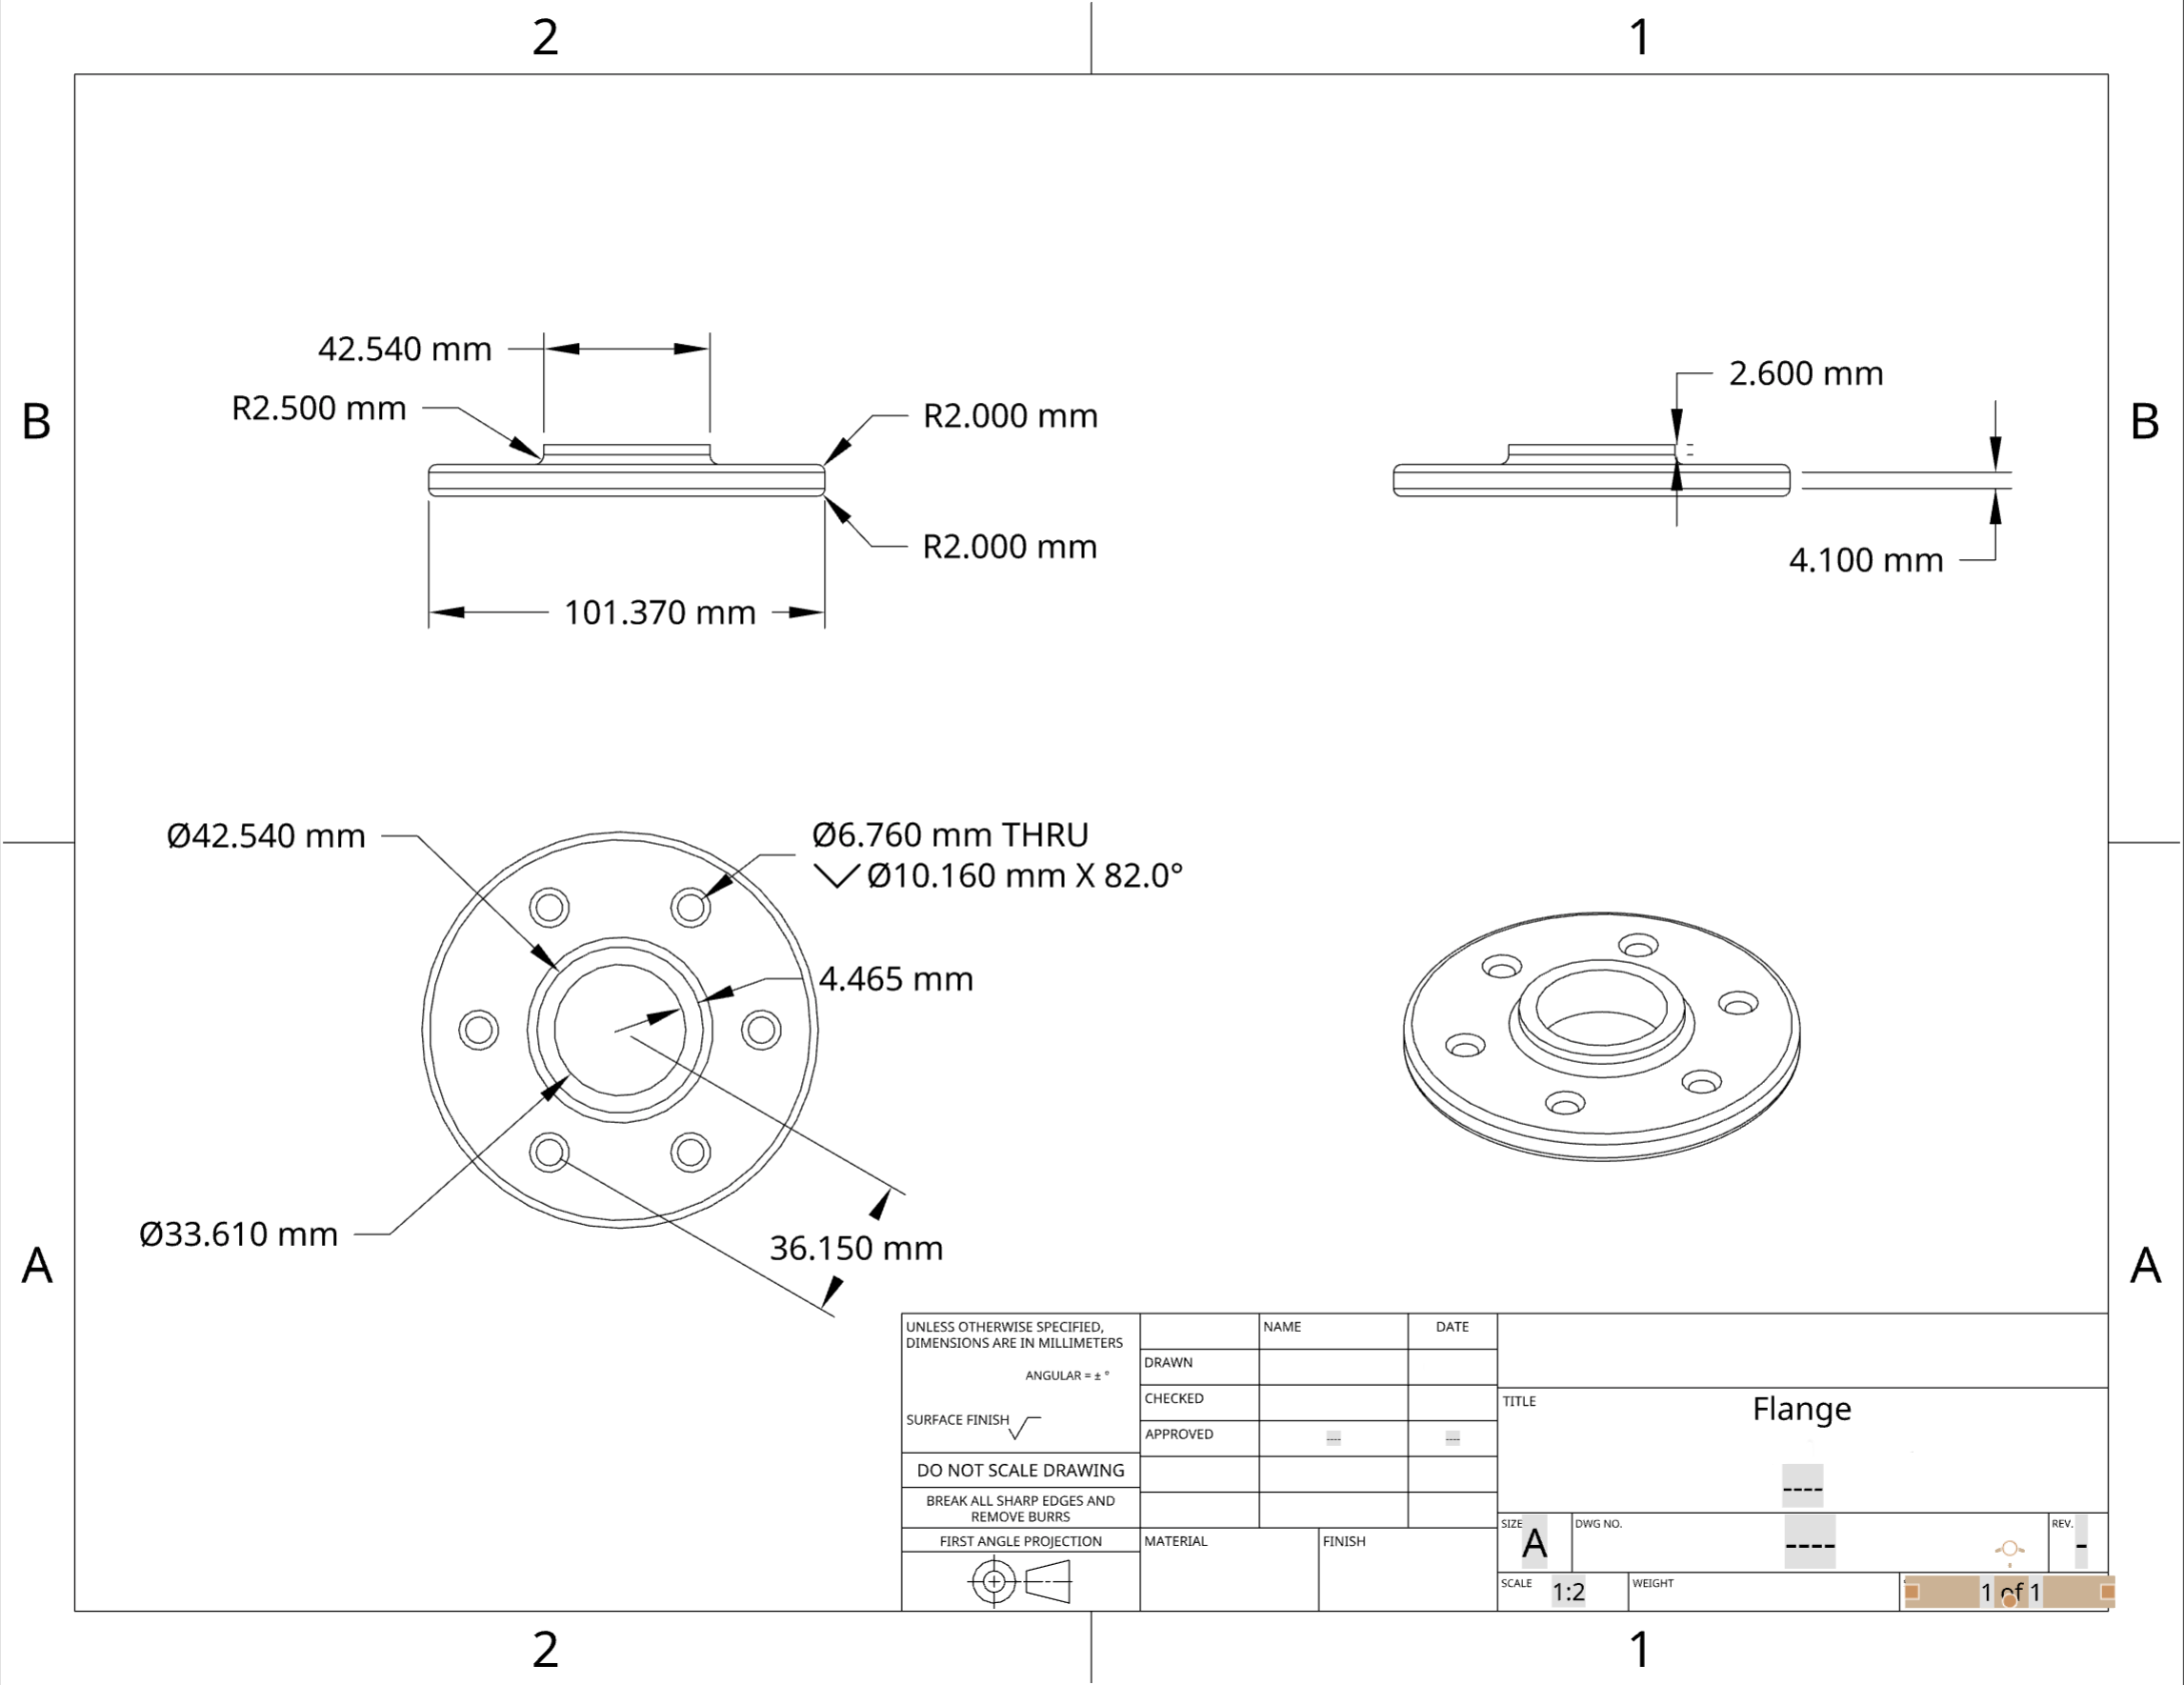
\includegraphics[width=1.0\textwidth]{FlangeMechanicalDrawing.png}}
    \centering{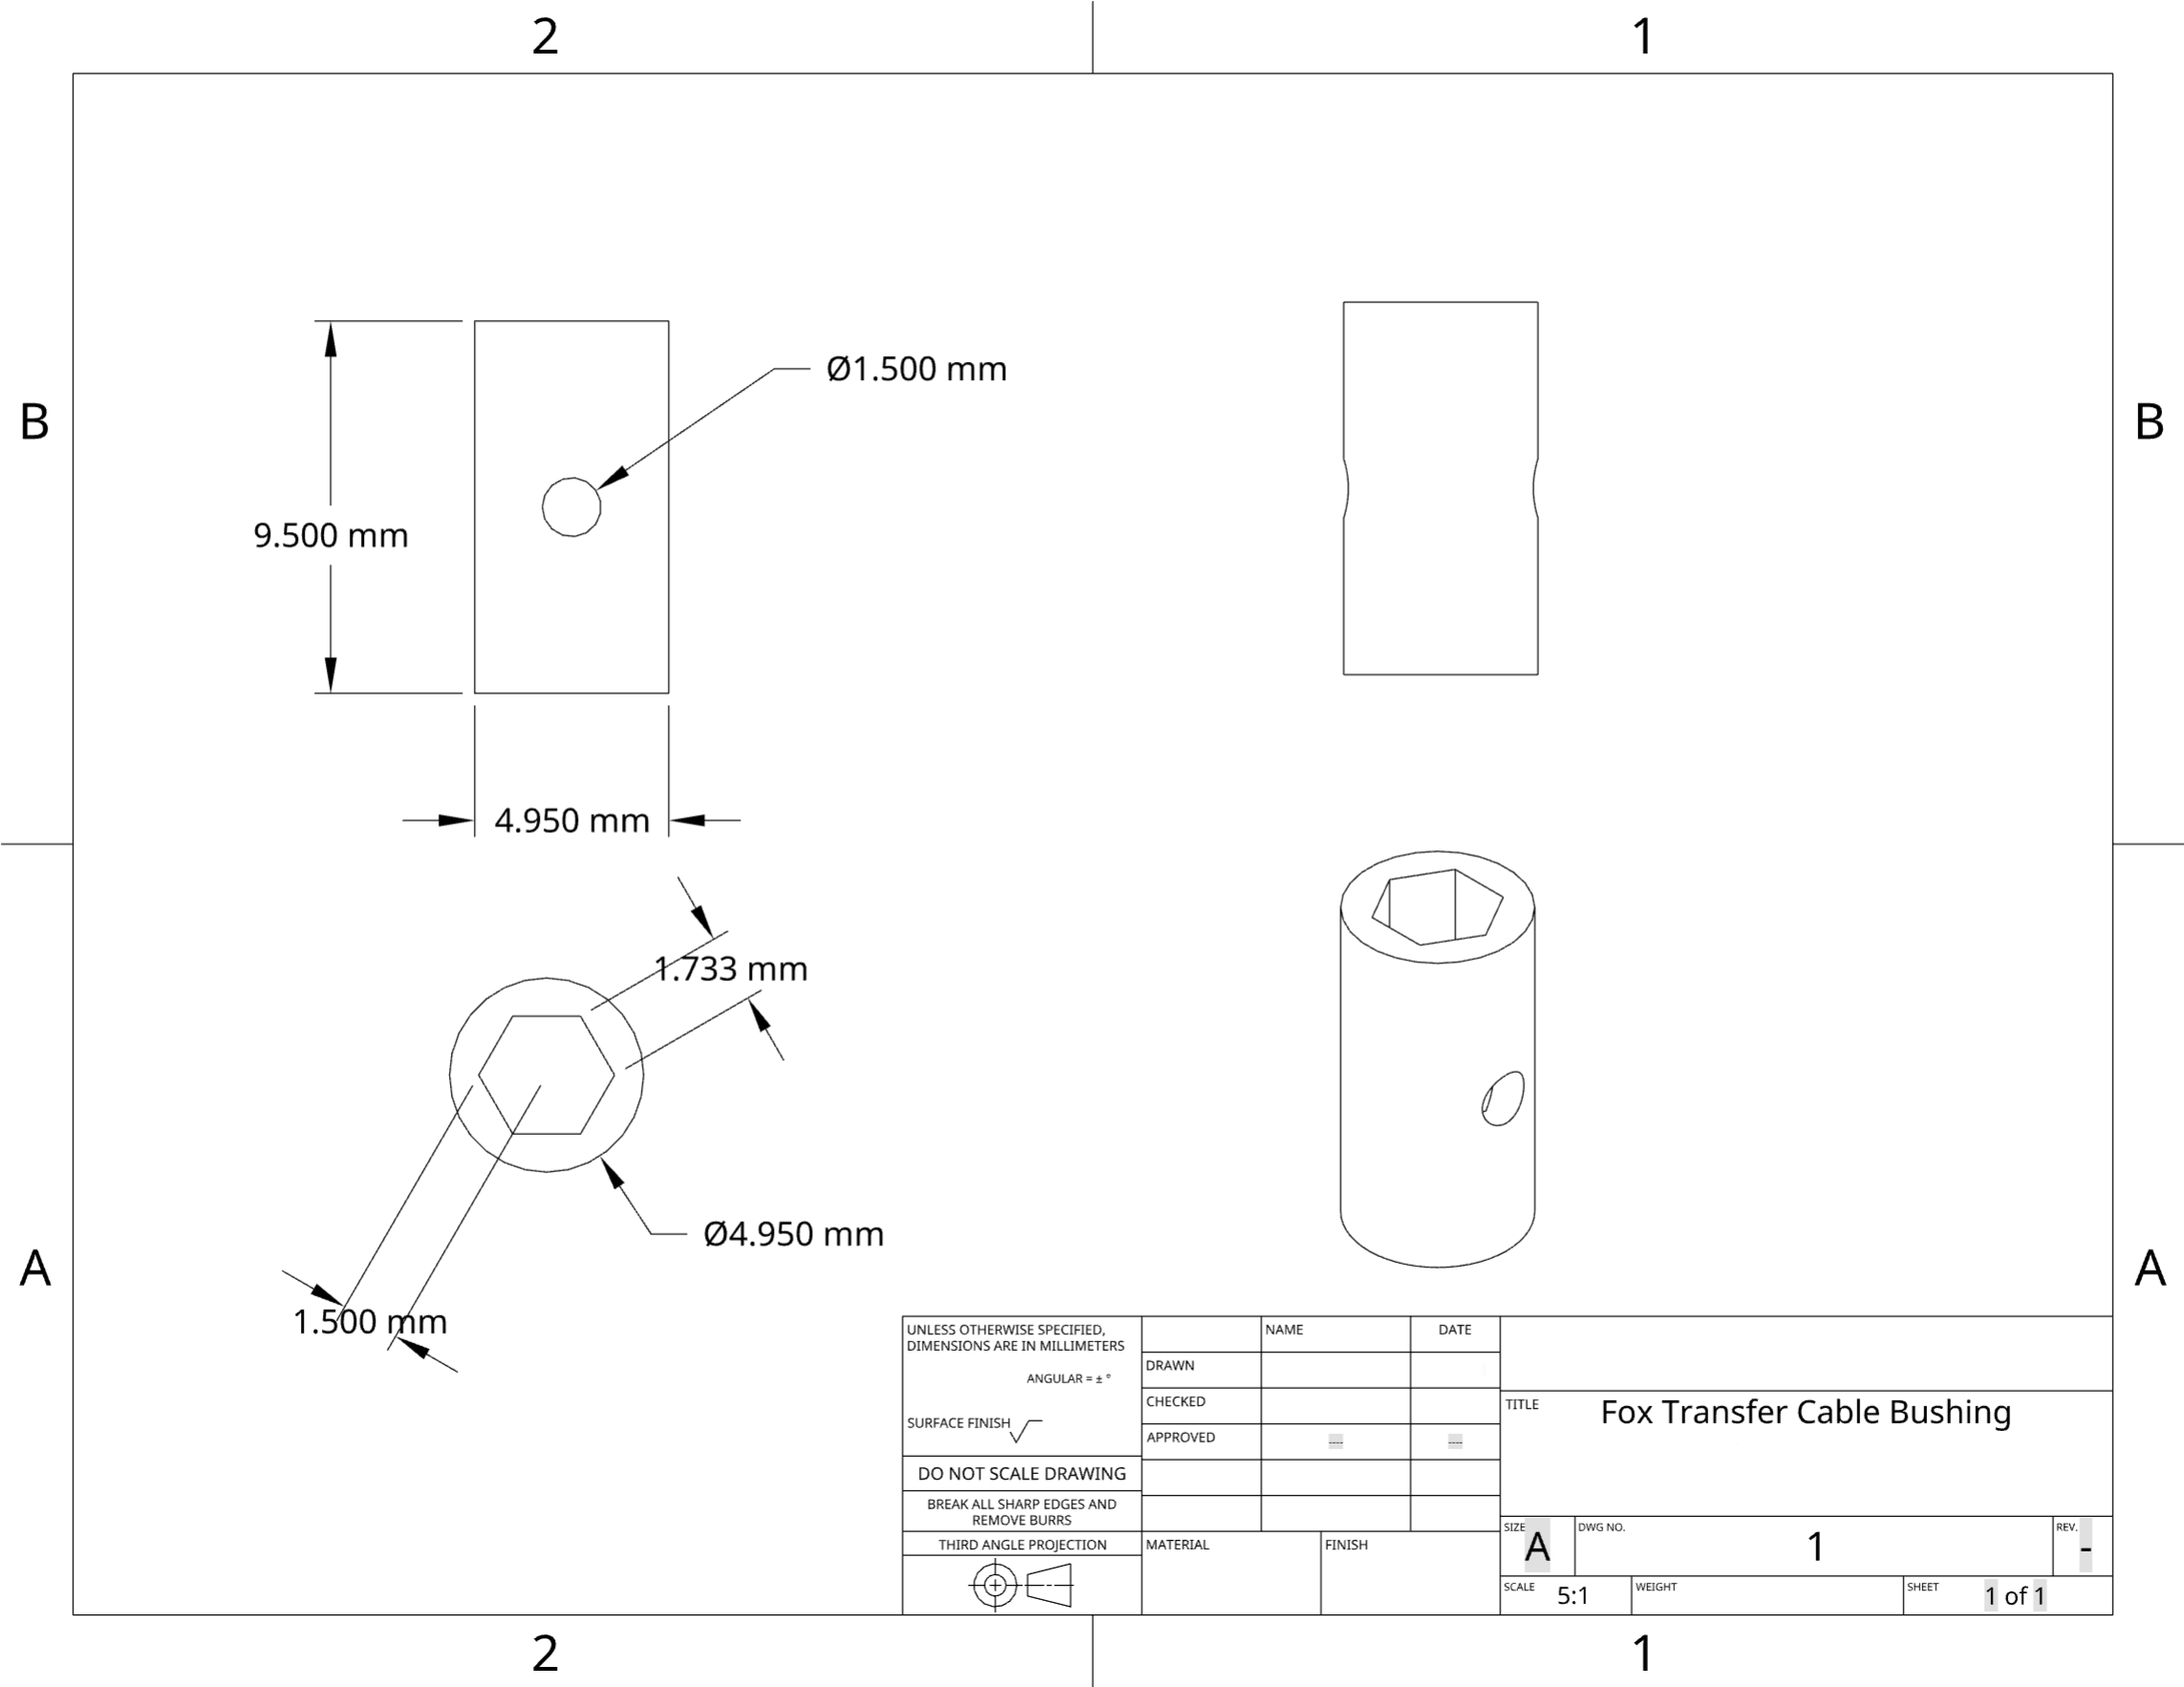
\includegraphics[width=1.0\textwidth]{FoxTransferCableBushing.png}}
\end{document}
